\section{Grundlagen neuronaler Netze}
\label{sec:neuronale-netze}

Neuronale Netze sind eine Modellklasse, welche zur L\"osung des
bereits ausf\"uhrlich
in~\cite{statistical_learning} beschriebenen Problems des statistischen
Lernens eingesetzt werden k\"onnen.
In dieser Problemsituation wird angenommen, dass sich der Zusammenhang zwischen
beobachtbaren Pr\"adiktorvariablen $X_1, ..., X_p$, welche sich durch
einen Vektor $X = (X_1, ..., X_p)$ zusammenfassen lassen, und einer
Zielvariable $Y$ durch eine Funktion $f^*$ mit $Y = f^*(X) + \epsilon$
modellieren l\"asst. Hierbei kann $\epsilon$ als eine zuf\"allige
St\"orgr\"o{\ss}e angesehen werden, die hier im weiteren Verlauf aber
keine wichtige Rolle spielt.
Das Ziel von neuronalen Netzen ist es, die unbekannte Funktion $f^*$
zu approximieren.

Damit $f^*$ approximiert werden kann, ist es notwendig, sowohl $X$
als auch $Y$ zu Beobachten. Ist dies geschehen, so liegen die
Beobachtungen in Form einer Menge von \textbf{Trainingsdaten}
$S$ vor, die sich wie folgt formalisieren l\"asst:
\begin{equation}
    \label{eq:trainingsdaten}
    S = \left\{ (x_1, y_1), ..., (x_n, y_n) \right\},
    \quad x_i \in \mathbb{R}^p, \  y_i \in \mathbb{R}^d, \  i=1, ..., n
\end{equation}
Die $x_i$ entsprechen hierbei den Beobachtungen des Zufallsvektors $X$
und die $y_i$ sind die Beobachtungen bez\"uglich $Y$.
Dem aufmerksamen Leser wird aufgefallen sein, dass die $y_i$ (und damit auch $Y$)
als Elemente des $\mathbb{R}^d$, also als $d$-dimensionale Vektoren
modelliert wurden, was eine Abweichung zum Modell aus~\cite{statistical_learning}
darstellt. Dies h\"angt mit der vorliegenden Datensituation dieses
Projektes zusammen.

Es kann an dieser Stelle n\"amlich schon vorweggenommen werden, dass es sich bei den
$x_i$ hier um Bilddaten handelt, und zwar um Bilder von Autos
mit Nummernschildern. Innerhalb der $y_i$ sollen dann sp\"ater
Informationen zur Position der Nummernschilder kodiert werden,
die durch das neuronale Netz vorhergesagt werden sollen.
Details zur Kodierung der $y_i$ und auch der $x_i$ sollen aber
an dieser Stelle bewusst noch
nicht vertieft werden, da zun\"achst die wichtigsten Grundlagen neuronaler
Netze entwickelt werden m\"ussen.

Die folgenden Erkl\"arungen zum Aufbau und zum Training neuronaler Netze
st\"utzen sich wesentlich auf~\cite{Goodfellow-et-al-2016} und sind hier
auf das grundlegendste reduziert worden.
Obwohl es der Name \textit{neuronale} Netze suggeriert, wird auch hier
genau wie in~\cite{Goodfellow-et-al-2016} ebenfalls auf jegliche
biologische Motivation verzichtet, damit nicht der falsche Eindruck
entstehen kann, dass es sich bei neuronalen Netzen um Modelle von echten
biologischen Gehirnen handelt.
Das Ziel von neuronalen Netzen ist es viel eher, unbekannte Funktionen
anhand von Trainingsdaten zu approximieren, um anschlie{\ss}end Vorhersagen
auf neuen und ungesehenen Daten anzustellen.

\subsection{Aufbau}
\label{sec:aufbau}

Wie oben in~\ref{sec:neuronale-netze} schon angedeutet, definiert ein neuronales Netz
also eine Abbildung $f$, welche den Zusammenhang zwischen einer Eingabe $x \in \mathbb{R}^p$
und einer Ausgabe $y \in \mathbb{R}^d$ approximieren soll.
Eine Hauptcharakteristik von neuronalen Netzen ist es, dass die Funktion $f$
durch die Verkettung weiterer Funktionen gebildet wird.
Ist ein neuronales Netz beispielsweise durch
$f(x) = f^{(3)}(f^{(2)}(f^{(1)}(x)))$ gegeben, so setzt es sich aus der
Verkettung der einzelnen Funktionen $f^{(1)}$, $f^{(2)}$ und
$f^{(3)}$ zusammen. Wie genau diese Funktionen aussehen k\"onnen, soll an dieser
Stelle bewusst ersteinmal offen bleiben.
Eine wichtige Voraussetzung an diese Funktionen ist allerdings die
Differenzierbarkeit, welche sp\"ater f\"ur das Training eines neuronalen
Netzes eine wichtige Rolle spielt.
Ansonsten ist es aber schon ausreichend, sich neuronale Netze als
Verkettungen (nahezu) beliebiger differenzierbarer Funktionen vorzustellen.

Solche Ketten von Funktionen k\"onnen gut durch gerichtete
azyklische Graphen beschrieben werden. Hierbei wird jedes Zwischenergebnis
durch einen Knoten repr\"asentiert, jede Kante zwischen zwei Knoten beschreibt
die Operation, die von einen Ergebnis zum n\"achsten gef\"uhrt hat.
Der Beispielgraph zu $f(x) = f^{(3)}(f^{(2)}(f^{(1)}(x)))$ ist in
Abbildung~\ref{fig:einfacher-graph} zu sehen.

\begin{figure}[h]
    \centering
    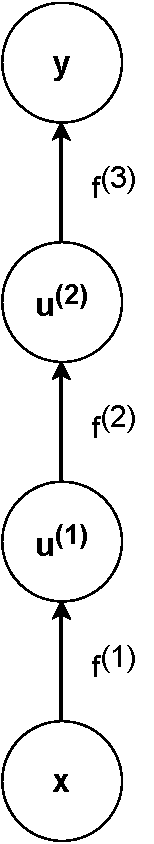
\includegraphics[height=0.3\textheight]{abbildungen/basic_network_graph}
    \caption{Verkettung dreier Funktionen dargestellt als
        gerichteter azyklischer Graph. Die Knoten $u^{(1)}$ und
        $u^{(2)}$ stellen die Zwischenergebnisse der Funktionen
        $f^{(1)}$ und $f^{(2)}$ dar, der Knoten $y$ repr\"asentiert
        die Ausgabe des Netzes.}
    \label{fig:einfacher-graph}
\end{figure}

Anhand dieses Beispielgraphen f\"allt auf, dass alle Pfeile in die
gleiche Richtung hin zur Ausgabe zeigen. Da eine Eingabe $x$ also
bildlich gesprochen immer in eine Richtung \textit{vorw\"arts} durch
den Graphen flie{\ss}t, spricht man hier auch von einem neuronalen
\textbf{feed-forward} Netz. Da diese Art von neuronalen Netzen in der
Praxis am h\"aufigsten vorkommt und auch in diesem Projekt verwendet
wurde, beschr\"anken sich alle folgenden Erkl\"arungen auf
feed-forward Netze.

Im Kontext von neuronalen Netzen wird jede der Funktionen
$f^{(1)}$, $f^{(2)}$ und $f^{(3)}$ auch als eine \textbf{Schicht} des
Netzes bezeichnet.
Da $f^{(1)}$ und $f^{(2)}$ im Inneren des Netzwerks liegen, bezeichnet man
diese Schichten auch als \textbf{versteckte Schichten}.
Die letzte Schicht eines neuronalen Netzes hingegen, also in diesem
Fall die Funktion $f^{(3)}$, wird als die \textbf{Ausgabeschicht} des
Netzwerks bezeichnet. Der Wert dieser Schicht ist gleichzeitig
auch der Ausgabewert des gesamten Netzes f\"ur eine Eingabe $x$.
Die Gesamtanzahl der Schichten eines neuronalen Netzes wird auch
als die \textbf{Tiefe} des Netzes bezeichnet.
Wie genau die Schichten eines neuronalen Netzwerkes nun aussehen k\"onnen,
soll im n\"achsten Abschnitt etwas detaillierter beschrieben werden.

\subsection{Schichten}
\label{sec:schichten}

Eine Schicht eines neuronalen Netzes ist eine Funktion $f$, die eine
Eingabe $x \in \mathbb{R}^n$ auf eine Ausgabe $f(x) \in \mathbb{R}^m$
abbildet. H\"aufig hat $f$ dabei die folgende Form:
\begin{equation}
    f(x) = g(Wx + b)
\end{equation}
$W \in \mathbb{R}^{m \times n}$ ist hierbei eine sogenannte Gewichtsmatrix,
die die Eingabe $x$ der Schicht linear transformiert.
Ist $W$ dicht besetzt, so spricht man auch von einer dichten
(eng. \textbf{dense}) Schicht.
$b \in \mathbb{R}^m$ wird auch Bias genannt und wird auf das Ergebnis der
Multiplikation von $W$ mit $x$ addiert.
Die Funktion $g: \mathbb{R}^m \rightarrow \mathbb{R}^m$ hei{\ss}t
Aktivierungsfunktion.

Oftmals ist es so, dass Aktivierungsfunktionen elementweise auf das
Resultat von $Wx + b$ angewendet werden. Hierzu kann man sich eine
Funktion $\Phi: \mathbb{R} \rightarrow \mathbb{R}$ definieren und dann
$g_i(u) = \Phi(u_i), \  i=1,...,m$ setzen. Hierbei beschreibt $g_i$
das $i$-te Element der vektorwertigen Funktion $g$ und $u_i$ das $i$-te
Element des Eingabevektors $u$ der Aktivierungsfunktion,
also in diesem Fall $u = Wx + b$.

F\"ur das sp\"ater in Abschnitt~\ref{sec:training} beschriebene
Training neuronaler Netze ist es wichtig, dass $f$ eine differenzierbare
Funktion ist. Damit dies gegeben ist, muss in diesem Fall also auch die
Aktivierungsfunktion $g$, beziehungsweise die elementweise angewendete
Funktion $\Phi$ differenzierbar sein.

Die Parameter $W$ und $b$ einer Schicht k\"onnen w\"ahrend der Trainingsphase
des neuronalen Netzwerks optimiert und an die Trainingsdaten
angepasst werden.
Die Aktivierungsfunktion einer Schicht hingegen ist ein sogenannter
\textbf{Hyperparameter} des Netzwerks. Dies bedeutet, dass dieser
Parameter vor dem Training vom Anwender spezifiziert werden muss.
Der Parameter $m$, also die Ausgabedimension der Schicht, ist ebenfalls
ein Hyperparameter.

\subsection{Aktivierungsfunktionen}

Im Folgenden werden ausschlie{\ss}lich elementweise Aktivierungsfunktionen
$\Phi: \mathbb{R} \rightarrow \mathbb{R}$ betrachtet,
da diese die gr\"o{\ss}te praktische Relevanz haben.
Zwei sehr h\"aufig eingesetzte Aktivierungsfunktionen, die auch in diesem
Projekt verwendet wurden, sind die \textbf{Rectified Linear Unit (ReLU)}
Funktion und die \textbf{Sigmoid} Funktion.
Beide werden im Folgenden kurz beschrieben.

\paragraph{ReLU}

Die ReLU Funktion ist nach~\cite{glorot} quasi eine
Standardempfehlung f\"ur die Aktivierungsfunktion in den
versteckten Schichten tiefer neuronaler Netze.
Sie ist durch folgenden Ausdruck gegeben:
\begin{equation*}
    \Phi_\text{ReLU}(x) = \max \{ 0, x \}
\end{equation*}
Wird diese Funktion elementweise auf einen Vektor angewendet, so werden
alle negativen Elemente auf Null gesetzt. Die restlichen Elemente bleiben
unber\"uhrt.
Dieses Vorgehen hat in der Praxis viele Vorteile~\cite{glorot}, unter
anderem erreicht man durch das Setzen negativer Eingaben auf 0,
dass Zwischenergebnisse im Netzwerk d\"unn besetzt sind, was das Training
der neuronalen Netze erleichtern kann.

Es f\"allt sofort auf, dass die ReLU Funktion im Punkt $x=0$ nicht
differenzierbar ist, was ja eigentlich f\"ur das Training neuronaler
Netze unerw\"unscht ist.
Dies stellt dank des Konzeptes von Subgradienten~\cite{understanding_ml}
(was hier bewusst nicht weiter vertieft werden soll)
aber in der Praxis kein Problem dar, da man den Wert der Ableitung der ReLU Funktion
an der Stelle $x=0$ in praktischen Implementierungen auf einen konstanten
Wert zwischen 0 und 1 setzen kann.

\paragraph{Sigmoid} Die Sigmoid Funktion ist durch folgenden Ausdruck gegeben:
\begin{equation*}
    \Phi_\text{Sigmoid}(x) = \frac{1}{1 + \exp{(-x)}}
\end{equation*}
Da der Wertebereich der Sigmoid Funktion auf das Intervall $[0, 1]$
beschr\"ankt ist, kommt diese Funktion h\"aufig in der Ausgabeschicht
von neuronalen Netzen zum Einsatz. Beispielsweise bietet es sich im
Szenario einer bin\"aren Klassifikation, also $y \in \{0, 1\}$, h\"aufig
an, die Sigmoidfunktion in der Ausgabeschicht zu verwenden.
Das weitere Vorgehen ist dann sehr \"ahnlich zur
logistischen Regression~\cite{statistical_learning}.

\subsection{Training}
\label{sec:training}

M\"ochte man ein neuronales Netz zur Approximation einer unbekannten
Funktion $f^*$ einsetzen, so muss man sich zun\"achst f\"ur eine
grundlegende Architektur des Netzes entscheiden.
Dies bedeutet, dass man festlegen muss, welche Art von Schichten wie
miteinander kombiniert werden sollen.
Je nach Anwendungsfall k\"onnen hier unterschiedliche Architekturen
sinnvoll sein und es m\"ussen oft mehrere Varianten getestet und
gegeneinander abgewogen werden.

Gehen wir aber nun einmal davon aus, dass wir uns f\"ur eine konkrete
Architektur entschieden haben (die tats\"achliche Architektur, die in
diesem Projekt zum Einsatz gekommen ist, wird sp\"ater beschrieben).
Die Frage ist nun, wie die freien Parameter, also die
Gewichtsmatrizen $W$ sowie die Bias Vektoren $b$ in jeder Schicht angepasst
werden k\"onnen, damit das neuronale Netz die Funktion $f^*$ m\"oglichst
gut approximiert.

Zur Beantwortung dieser Frage ist es hilfreich, sich in Erinnerung
zu rufen, dass ein neuronales Netz lediglich durch eine Funktion
$f(x)$ von einer Eingabe $x$ beschrieben werden kann.
S\"amtliche Parameter dieser Funktion (also die Gewichtsmatrizen und
die Bias-Vektoren) lassen sich o.B.d.A. zu einem einzigen
Parametervektor $\theta$ zusammenfassen, welcher die Funktion $f$
parametrisiert (wir sprechen deshalb im Folgenden von $f_\theta$).

Der mittlere quadratische Approximationsfehler unseres neuronalen Netzes
$f_\theta$ f\"ur einen Parametervektor $\theta$ auf den bereits
in Gleichung~\ref{eq:trainingsdaten} beschriebenen Trainingsdaten $S$
l\"asst sich dann wie folgt berechnen:
\begin{equation}
    L(\theta) = \frac{1}{n} \sum_{i=1}^n \left\lVert y_i - f_\theta(x_i) \right\lVert_2^2
\end{equation}

Das Training eines neuronalen Netzes $f_\theta$ besteht nun also darin,
einen Parametervektor $\theta$ zu finden, f\"ur den die sogenannte
Verlustfunktion $L(\theta)$ minimiert wird.
Es liegt also ein nicht-lineares Optimierungsproblem einer geschlossenen
und differenzierbaren Funktion $L(\theta)$ vor.

Zur L\"osung eines solchen Problems gibt es viele verschiedene Verfahren.
In der Praxis kommen meist Varianten des stochastischen Gradientenabstiegs
zum Einsatz. Dieses allgemeine Optimierungsverfahren ist in~\cite{understanding_ml}
im Bezug auf allgemeine Machine Learning Probleme ausf\"uhrlich beschrieben
und analysiert worden und soll hier nur einmal bez\"uglich der
vorliegenden Problemstellung kurz umrissen werden.

\paragraph{Stochastischer Gradientenabstieg}

M\"ochte man die Funktion $L(\theta)$ durch stochastischen Gradientenabstieg
minimieren, so muss man zun\"achst einen Startwert $\theta^{(0)}$
ausw\"ahlen, an welchem die Optimierung beginnen soll.
Hierbei gibt es viele m\"ogliche Vorgehensweisen.
Im Kontext tiefer neuronaler Netze hat sich beispielsweise die
Glorot Initialisierung bew\"ahrt, welche erstmals in~\cite{glorot_init}
vorgestellt wurde und auf eine zuf\"allige, aber m\"oglichst gleichm\"a{\ss}ige
Initialisierung der Parameter abzielt.

Hat man einen Startwert $\theta^{(0)}$ gew\"ahlt, so wird dieser nun
durch stochastischen Gradientenabstieg schrittweise verbessert.
Dies geschieht dadurch, dass sukkzessive Schritte in die Richtung
des negativen Gradienten von $L(\theta)$ durchgef\"uhrt werden.
Im Optimierungsschritt $t$ wird der aktuelle Parametervektor $\theta^{(t)}$
also wie folgt aktualisiert:
\begin{equation}
    \theta^{(t+1)} = \theta^{(t)} - \eta \nabla L(\theta^{(t)})
\end{equation}
Hierbei gibt $\eta$ eine Schrittweite an, die zuvor vom Anwender
spezifiziert werden muss.

Die Idee dabei ist, dass der negative Gradient immer in die Richtung
des steilsten Abstieges einer Funktion zeigt.
Man erhofft sich durch diese lokale Minimierung der Funktion, dass
man schlussendlich in einem globalen Minimum auskommt. Dies ist aber nur
dann mathematisch garantiert, wenn die Funktion $L(\theta)$ konvex ist
(in diesem Fall gibt es nur ein einziges globales Minimum).
Da es sich hier allerdings um ein hochgradig nicht-lineares Optimierungsproblem
handelt, ist die Konvexit\"at von $L$ f\"ur tiefe neuronale Netze in den
meisten F\"allen nicht gegeben. Man kann also bestenfalls auf die Konvergenz
des Verfahrens in ein lokales Minimum hoffen.
Laut~\cite{local_minima} scheint es aber in der Praxis Anhaltspunkte
daf\"ur zu geben, dass lokale Minima anders als man denken k\"onnte
oft kein gro{\ss}es Problem beim Training darstellen.

\paragraph{Berechnung der Gradienten}

Eine weitere offene Frage ist, wie der Gradient von $L$ berechnet werden
kann. Hierbei hilft es, sich erneut in Erinnerung zu rufen, dass es sich
bei $L$ und auch bei $f_\theta$ um geschlossene Funktionen handelt,
deren Gradienten explizit angegeben werden k\"onnen.
Dennoch bleibt die Frage, wie dies algorithmisch effizient umgesetzt werden
kann.

In der Praxis kommt hier meist der sogenannte
Backpropagation-Algorithmus~\cite{backpropagation} zum Einsatz.
Eine detaillierte Beschreibung dieses Algorithmus' w\"urde an dieser
Stelle zu weit f\"uhren, die Grundidee jedoch l\"asst sich in wenigen
S\"atzen beschreiben.

Wie bereits in Abschnitt~\ref{sec:aufbau} und insbesondere anhand von
Abbildung~\ref{fig:einfacher-graph} gezeigt, lassen sich neuronale Netze
als Verkettungen von Funktionen beschreiben, die durch
azyklische Graphen dargestellt werden k\"onnen.
Die Verlustfunktion, deren Gradient berechnet werden soll, l\"asst sich
ebenfalls durch einen solchen Graphen beschreiben.
Der Backpropagation-Algorithmus ist ein allgemeines Verfahren, welches den
Gradienten von
Funktionen, die durch azyklische Graphen beschrieben werden k\"onnen,
durch Anwendung der \textbf{Kettenregel} berechnen kann.

Die Details werden hier bewusst ausgespart, es soll allerdings betont
werden, dass es sich beim Backpropagation-Algorithmus lediglich um eine
effiziente Berechnungsvorschrift der Kettenregel handelt.
Bekannte Programmbibliotheken wie Tensorflow~\cite{tensorflow2015-whitepaper}
implementieren dieses Verfahren durch effiziente Ausnutzung vorhandener
Hardware (insbesondere GPUs) und erfreuen sich daher
gro{\ss}er Beliebtheit.

\subsection{Convolutional Neural Networks}

Convolutional Neural Networks (im folgenden \textbf{CNN}) sind eine
spezielle Art von neuronalen feed-forward Netzen, die sich besonders f\"ur den
Einsatz auf Bilddaten eignen~\cite{Goodfellow-et-al-2016}.
Der Name r\"uhrt daher, dass CNNs in mindestens einer ihrer Schichten
eine sogenannte Faltungsoperation (eng. Convolution) verwenden.

Eine detaillierte und formale Beschreibung der Faltungsoperation w\"urde
hier an dieser Stelle zu weit f\"uhren. Daher wird im folgenden
die Funktionsweise einer sogenannten \textbf{Faltungsschicht} eines
CNNs lediglich kurz intuitiv umrissen. F\"ur mehr Details wird auf
Fachliteratur wie~\cite{Goodfellow-et-al-2016} verwiesen.

\paragraph{Faltungsschichten}

\begin{figure}[h]
    \centering
    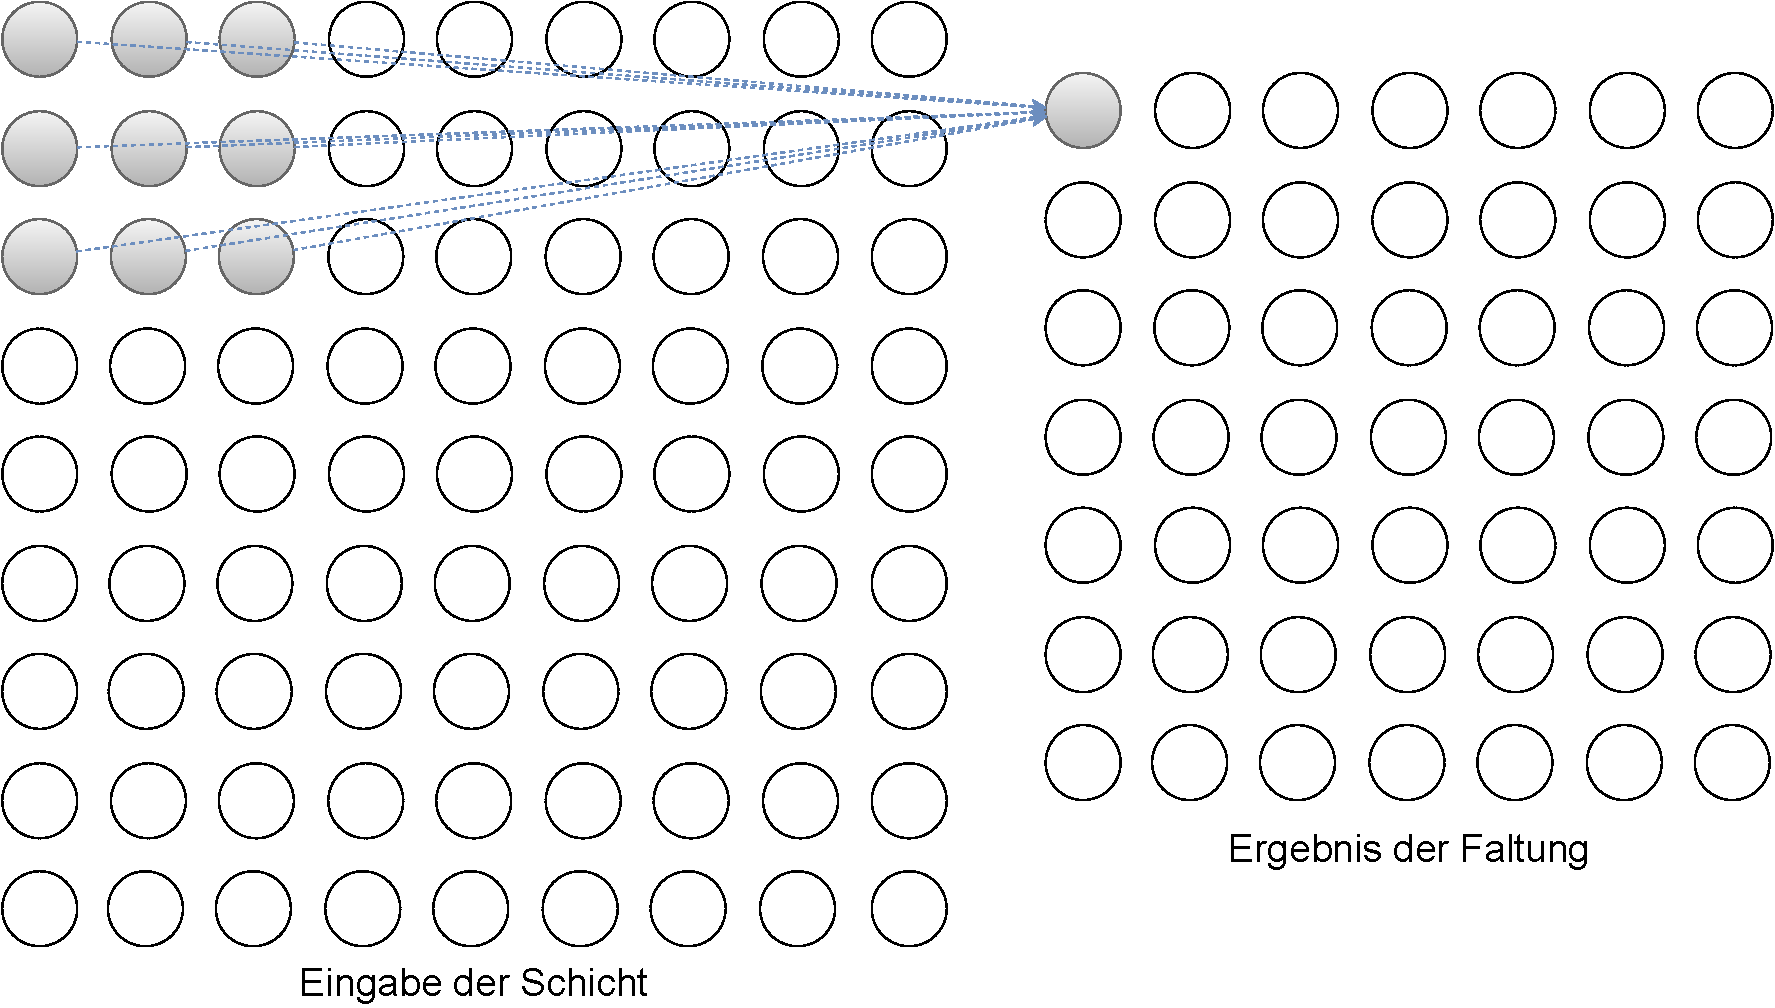
\includegraphics[width=0.9\textwidth]{abbildungen/faltungsschicht}
    \caption{Schematische Darstellung einer Faltungsschicht}
    \label{fig:faltungsschicht}
\end{figure}

Eine schematische Darstellung einer Faltunsschicht ist in
Abbildung~\ref{fig:faltungsschicht} gegeben.
Der erste Unterschied zur bereits in~\ref{sec:schichten} beschriebenen
dense Schicht ist, dass die Eingabe eine zweidimensionale Struktur
aufweist, wie es beispielsweise bei (schwarz-wei{\ss}en) Bilddaten der Fall ist.
Zur formalen Beschreibung solcher Daten k\"onnen beispielsweise anstelle
von Vektoren Matrizen zum Einsatz kommen. In Abbildung~\ref{fig:faltungsschicht}
w\"urde dann jeder Punkt im linken Gitter einem Eintrag aus der Eingabematrix der
Schicht entsprechen.\footnote{In der Praxis wird dieses Konzept h\"aufig auf
    mehr als zwei Dimensionen verallgemeinert. Dies ist insbesondere
    dann n\"otig, wenn man es beispielsweise mit Farbbildern zu tun hat,
    die f\"ur jeden Pixel drei Farbwerte speichern. In diesem Fall spricht man
    dann nicht mehr von Matrizen, sondern von \textbf{Tensoren}.}

Die Faltungsoperation auf einer solchen Eingabe kann man sich nun so
vorstellen, dass eine Art Fenster (auch \textbf{Kernel} genannt)
Schritt f\"ur Schritt \"uber die Eingabe f\"ahrt und dabei eine gewichtete
Summe berechnet. In Abbildung~\ref{fig:faltungsschicht} hat dieses Fenster
die Gr\"o{\ss}e 3x3, die gewichtete Summe wird durch die blauen Pfeile
symbolisiert. Analog zur dense Schicht wird zudem auf jedes Ergebnis
der gewichteten Summe ein Bias aufaddiert. Im Anschluss wird auch bei
Faltunsschichten auf die Ausgabe eine (meist elementweise)
Aktivierungsfunktion angewendet.

Die Gewichte des Kernels zusammen mit dem Bias und der
Aktivierungsfunktion sind die trainierbaren
Parameter einer Faltungsschicht. Die Kernel-Gr\"o{\ss}e, sowie die
Schrittweite, mit welcher der Kernel \"uber die Eingabe f\"ahrt,
sind Hyperparameter, die vom Anwender vor dem Training spezifiziert werden
m\"ussen.
Es ist dar\"uber hinaus bei Faltungsschichten auch \"ublich, gleich
mehrere Kernel gleichzeitig einzusetzen. Auf diese Weise erh\"alt man
dann auch mehrere Ausgabematrizen, die dann \"ubereinander geschichtet
werden k\"onnen (man erh\"alt also einen Ausgabe\textbf{tensor}).
Die Anzahl der Kernel einer Faltungsschicht ist ebenfalls
ein Hyperparameter.

\paragraph{Pooling und Upsampling Schichten}

Zwei weitere Arten von Schichten, die oft in CNNs zum Einsatz kommen und
auch in diesem Projekt angewendet wurden, sind Pooling und Upsampling
Schichten. Beide sind in Abbildung~\ref{fig:pooling} schematisch
dargestellt.

\begin{figure}[h]
    \centering
    \begin{subfigure}{0.45\textwidth}
        \centering
        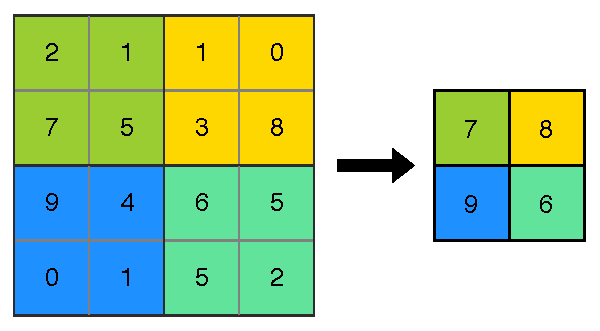
\includegraphics[width=\textwidth]{abbildungen/pooling}
        \subcaption{Max-Pooling}
    \end{subfigure}
    \unskip\ \vrule\
    \begin{subfigure}{0.45\textwidth}
        \centering
        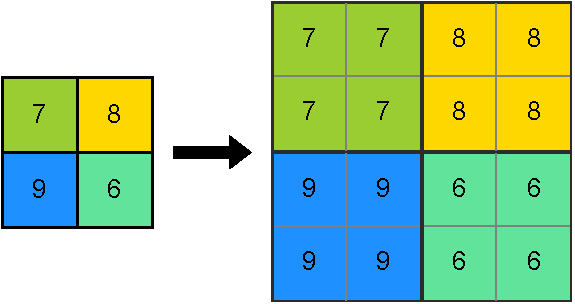
\includegraphics[width=\textwidth]{abbildungen/upsampling}
        \subcaption{Upsampling}
    \end{subfigure}
    \caption{Die Pooling Schicht (links) reduziert die Dimension ihrer
        Eingabe, die Upsampling Schicht (rechts) bewirkt das Gegenteil.}
    \label{fig:pooling}
\end{figure}

Die Aufgabe von Pooling Schichten innerhalb eines CNN ist es, die
dimensionalit\"at ihrer Eingabe zu verringern. Pooling Schichten verf\"ugen
\"uber keine trainierbaren Parameter.
\"Ahnlich zu Faltungsschichten basieren auch Pooling Schichten auf
einem Kernel, der \"uber die Eingabe f\"ahrt. Der Unterschied ist aber,
dass der Kernel keine gewichtete Summe berechnet, sondern lediglich
das Maximum zur\"uckgibt.\footnote{In diesem Fall spricht man auch von
    Max-Pooling. Bei einer anderen Variante, dem Average-Pooling, wird die
    Eingabe des Kernels auf den Durchschnitt reduziert.}
Au{\ss}erdem ist es im Falle von Pooling \"ublich, dass der Kernel
gr\"o{\ss}ere Schritte zur\"ucklegt. Im Beispiel von
Abbildung~\ref{fig:pooling} ist die Kernel-Gr\"o{\ss}e 2x2 und die
Schrittweite 2. So wird die Eingabe von 4x4 auf 2x2 reduziert, die
Dimensionalit\"at wird also halbiert.

Upsampling Schichten sind in gewisser Weise die Gegenspieler von
Pooling Schichten, da sie die Dimensionalit\"at ihrer Eingabe
k\"unstlich vergr\"o{\ss}ern, indem sie jeweils Zeilen und
Spalten vervielfachen (in Abbildung~\ref{fig:pooling} werden sowohl
Zeilen als auch Spalten verdoppelt).
Auch Upsampling Schichten haben keine trainierbaren Parameter.
